\documentclass[journal,trans]{IEEEtran}
\usepackage[spanish]{babel}
\usepackage[utf8]{inputenc}
\usepackage{graphicx}
\usepackage[dvipsnames]{xcolor}
\usepackage{multirow}
\usepackage{amsmath}
\usepackage{amssymb}
%\usepackage[spanish,activeacute]{babel}
%\usepackage[english,spanish]{babel}
%\usepackage{ifpdf}
\usepackage{cite}
%\usepackage[cmex10]{amsmath}
\usepackage{url}
\hyphenation{op-tical net-works semi-conduc-tor}

\begin{document}
	
	\newcommand{\titlepaper}{Laboratorio 4: Lógica Secuencial y Controladores}
	
	\title{\titlepaper}
	
	\renewcommand\IEEEkeywordsname{Palabras clave}
	
	\author{\IEEEauthorblockN{Fiorella Delgado León, Jonathan Guzmán Araya, Gerald Valverde Mc kenzie}
		\IEEEauthorblockA{\\fiorelladelgado53@gmail.com, jonathana1196@gmail.com, gvmckenzie@mckode.com}
		\IEEEauthorblockA{\\Área Académica de Ingeniería en Computadores}
		\IEEEauthorblockA{\\Instituto Tecnológico de Costa Rica, Cartago, Costa Rica, 2021}
	}
	
	\markboth{Taller de Diseño Digital, \titlepaper}%
	{Shell \MakeLowercase{\textit{et al.}}: Bare Demo of IEEEtran.cls for Journals}
	
	% Note that keywords are not normally used for peerreview papers.
	
	\IEEEtitleabstractindextext{%
		\begin{abstract}
			In this laboratory it´s put into practice the work with FPGAs, their respective configuration in the System Verilog and VHDL language also an introduction to VGA controllers was made, as well as the concept of finite state machines was remembered and used both in its behavioral and structural form in VHDL for problem solving.
		\end{abstract}
		\begin{IEEEkeywords}
			Backtracking, clock, comportamiento, controladores, estructural, Flip-Flop, FPGA, FSM, reset, RGB, síntesis lógica y testbench. VGA.
	\end{IEEEkeywords}}
	
	% make the title area
	\maketitle
	
	\IEEEdisplaynontitleabstractindextext
	
	\IEEEpeerreviewmaketitle
	
	\section{Introducción}
	
	Un circuito secuencial es aquel en el cual las salidas en un instante de tiempo determinado son una función de las entradas en ese instante y en instantes anteriores, por lo que se dice que este tipo de circuitos es capaz de “memorizar” información.
	
	Una máquina de estados finitos es un modelo matemático de computación en un momento dado del tiempo, se encuentra en un estado, y realiza cómputos de forma automática sobre una entrada para producir una salida. Este modelo está conformado por un alfabeto $\Sigma$, un conjunto de estados finitos $Q$, una función de transición $\delta$, un estado inicial $q_{i} \in Q$, una posible función de salida $\Omega$, y un conjunto de estados finales $A$. 
	Su funcionamiento se basa en su función de transición, que recibe a partir de un estado inicial y que va avanzando en el autómata de un estado a otro causando una transición entre los estados dependiendo de la entrada que recibe, para finalmente detenerse en un estado final.
	La función de transferencia de una máquina de estados puede ser parcial, es decir, puede no estar definida para toda combinación de $q \in Q$  y $\sigma \in \Sigma$.
	
	El origen de los autómatas finitos probablemente se remonta a su uso implícito en máquinas electromecánicas, desde principios del siglo XX \cite{wolfram}.  Ya en 1907, el matemático ruso Andréi Márkov formalizó un proceso llamado cadena de Markov, donde la ocurrencia de cada evento depende con una cierta probabilidad del evento anterior \cite{vasharin} . Esta capacidad de "recordar" es utilizada posteriormente por los autómatas finitos, que poseen una memoria primitiva similar, en que la activación de un estado también depende del estado anterior, así como del símbolo o palabra presente en la función de transición.
	Posteriormente, en 1943, surge una primera aproximación formal de los autómatas finitos con el modelo neuronal de McCulloch-Pitts. Durante la década de 1950 prolifera su estudio, frecuentemente llamándoles máquinas de secuencia; se establecen muchas de sus propiedades básicas, incluyendo su interpretación como lenguajes regulares y su equivalencia con las expresiones regulares \cite{wolfram}. Al final de esta década, en 1959, surge el concepto de autómata finito no determinista en manos de los informáticos teóricos Michael O. Rabin y Dana Scott.
	En la década de 1960 se establece su conexión con las series de potencias y los sistemas de sobre-escritura. Finalmente, con el desarrollo del sistema operativo Unix en la década de 1970, los autómatas finitos encuentran su nicho en el uso masivo de expresiones regulares para fines prácticos, específicamente en el diseño de analizadores léxicos, la búsqueda y reemplazo de texto.	
	
	Se pueden clasificar en:
	
	\begin{itemize}
		\item Deterministas
		\begin{itemize}
			\item La transición desde un estado puede tener como destino un único estado.
			\item No se aceptan transiciones con cadenas vacías.
			\item Se permite el uso de backtracking.
			\item Una cadena es aceptada si su transición es hacia un estado final.
		\end{itemize}
		\item No deterministas
		\begin{itemize}
			\item La transición desde un estado puede tener múltiples destinos.
			\item Permite transiciones con cadenas vacías.
			\item Una cadena es aceptada si solo una de todas sus posibles transiciones son hacia un estado final.
		\end{itemize}
	\end{itemize}
	
	Adicionalmente, las máquinas de estado pueden ser clasificadas como Máquinas de Mealy, cuya salida depende de su estado actual y de la entrada, es decir $\Omega: Q \times \Sigma \to \Lambda$ ó Máquinas de Moore, cuya salida depende solamente de su estado actual, es decir $\Omega: Q \to \Lambda$.
	
	Los autómatas finitos se pueden representar mediante grafos particulares, también llamados diagramas de estados finitos, de la siguiente manera:
	
	\begin{itemize}
		\item Los estados \emph{Q} se representan como vértices, etiquetados con su nombre interior.
		\item Una transición $\delta$ desde un estado a otro, dependiente de un símbolo del alfabeto, se representa mediante una arista dirigida que une a estos vértices, y que no está etiquetada con dicho símbolo.
		\item El estado inicial $q_{0}$ se caracteriza por tener una arista que llega a él, proveniente de ningún otro vértice.
		\item El o los estados finales \emph{F} se representan mediante vértices que están encerrados a su vez por otra circunferencia.
	\end{itemize}
	
	El autómata finito en la Figura \ref{fig:FSME} está definido sobre el alfabeto ${\Sigma}=\{0,1\}$, posee dos estados, $S_{1}$ y $S_{2}$, y sus transiciones son ${\delta}(S_{1}, 0)=S_{2}$, ${\delta}(S_{1}, 1)=S_{1}$, ${\delta}(S_{2}, 0)=S_{1}$, y ${\delta}(S_{1}, 1)=S_{2}$. Su estado inicial es $S_{1}$, que también es su único estado final.
	
	
	\begin{figure}[h]
		\centering
		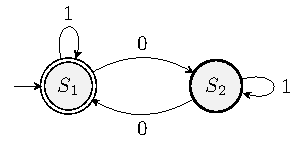
\includegraphics{./imagenes/FSME.pdf}
		\caption{Autómata que determina si un número binario tiene un cantidad par de ceros}
		\label{fig:FSME}
	\end{figure}
	
	Otra manera de describir el funcionamiento de un autómata finito es mediante el uso de tablas de transiciones o matrices de estados. Para el ejemplo de la Figura \ref{fig:FSME} la Tabla \ref{tab:FSME} y la Tabla \ref{tab:FSMT} son posibles representaciones alternativas.
	
	\begin{table}[h]
		\centering
		\begin{tabular}{||c|c|c||}
			\hline
			\hline
			Salida $q \in Q$ & Símbolo $\sigma \in \Sigma$ & Llegada $\delta (q, \sigma) \in Q$ \\
			\hline
			$S_{1}$          & 0                           & $S_{2}$\\
			$S_{1}$          & 1                           & $S_{1}$\\
			$S_{2}$          & 0                           & $S_{1}$\\
			$S_{2}$          & 1                           & $S_{2}$\\
			\hline
			\hline
		\end{tabular}
		\caption{Tabla de transiciones}
		\label{tab:FSME}
	\end{table}
	
	\begin{table}[h]
		\centering
		\begin{tabular}{||c|c|c||}
			\hline
			\hline
			&  0      & 1\\
			\hline
			\hline
			${\to} {\star} S_{1}$ & $S_{2}$ & $S_{1}$\\
			\hline
			$S_{2}$               & $S_{1}$ & $S_{2}$\\
			\hline
			\hline
		\end{tabular}
		\caption{Tabla de transiciones}
		\label{tab:FSMT}
	\end{table}
	
	En la Tabla \ref{tab:FSMT} se marca el estado inicial con $\to$ y el estado final con $\star$, mientras que en la tabla se muestra el estado actual y la entrada que causa la transición al siguiente estado.
	
	\vspace{4mm}
	
	La Figura \ref{figmachineMoore} muestra una máquina de Moore; un tipo de máquina de estados finitos que genera una salida basándose en su estado actual, para cada estado $S$, la salida aparece en el nodo, por ejemplo, para el estado \emph{A}, la salida 0 aparece como A/0. Para este ejemplo, se muestra una red secuencial, que tiene una entrada, y una salida. La salida es 1, y se mantiene en 1, cuando se han introducido al menos dos 0s, y dos 1s como entrada.
	
	\begin{figure}[h]
		\centering
		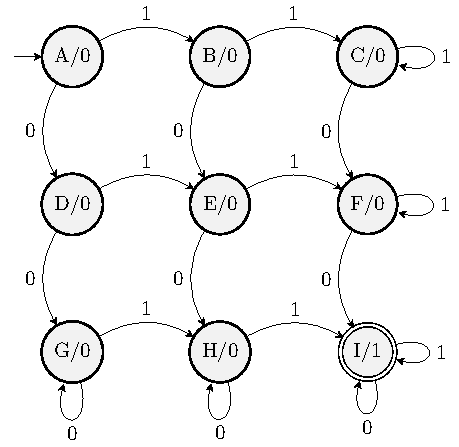
\includegraphics{./imagenes/machineMoore.pdf}
		\caption{Diagrama de estados de una máquina de Moore}
		\label{figmachineMoore}
	\end{figure}
	
	\begin{table}[h]
		\centering
		\bgroup
		\def\arraystretch{1.5}
		\begin{tabular}{|c|c|c|c|}
			\hline
			Estado actual & entrada & Siguiente estado & Salida \\
			\hline
			\multirow{2}{*}{A} & 0 & D & \multirow{2}{*}{0} \\
			\cline{2-3}
			& 1 & B & \\
			\hline
			\multirow{2}{*}{B} & 0 & E & \multirow{2}{*}{0} \\
			\cline{2-3}
			& 1 & C & \\
			\hline
			\multirow{2}{*}{C} & 0 & F & \multirow{2}{*}{0} \\
			\cline{2-3}
			& 1 & C & \\
			\hline
			\multirow{2}{*}{D} & 0 & G & \multirow{2}{*}{0} \\
			\cline{2-3}
			& 1 & E & \\
			\hline
			\multirow{2}{*}{E} & 0 & H & \multirow{2}{*}{0} \\
			\cline{2-3}
			& 1 & F & \\
			\hline
			\multirow{2}{*}{F} & 0 & I & \multirow{2}{*}{0} \\
			\cline{2-3}
			& 1 & F & \\
			\hline
			\multirow{2}{*}{G} & 0 & G & \multirow{2}{*}{0} \\
			\cline{2-3}
			& 1 & H & \\
			\hline
			\multirow{2}{*}{H} & 0 & H & \multirow{2}{*}{0} \\
			\cline{2-3}
			& 1 & I & \\
			\hline
			\multirow{2}{*}{I} & 0 & I & \multirow{2}{*}{1} \\
			\cline{2-3}
			& 1 & I & \\
			\hline
		\end{tabular}
		\egroup
		\caption{Tabla de Transición de red secuencial, cuya salida es 1 cuando ha tenido dos 0s y dos 1s de entrada}
		\label{tab:MooreTable}
	\end{table}
	
	Como se puede ver en la Tabla \ref{tab:MooreTable}, el valor de la salida solamente depende del estado actual.
	
	En contraste, como se puede ver en la Tabla \ref{tab:tableMealy}, el valor de la salida depende tanto del estado actual, como de la entrada, a excepción de la transición del estado inicial $S_{i}$, pero eso se debe al ejemplo particular.
	
	La Figura \ref{fig:machineMealy} muestra una máquina de Mealy; un tipo de máquina de estados finitos que genera una salida basándose en su estado actual y una entrada. Su diagrama de estados incluye ambas señales de entrada (en \textcolor{red}{rojo}) y de salida (en \textcolor{green}{verde}) para cada línea de transición. Esta empieza en el estado $S_{i}$, e implementa la función \emph{XOR} de los últimos dos valores m\'as recientemente introducidos.
	
	En contraste, la salida de una máquina de Moore de estados finitos (el otro tipo) depende solamente del estado actual de la máquina, dado que las transiciones no tienen entrada asociada. Sin embargo, para cada máquina de Mealy hay una máquina de Moore equivalente cuyos estados son la unión de los estados de la máquina de Mealy y el producto cartesiano de los estados de la máquina de Mealy y el alfabeto de la entrada.
	
	\begin{figure}[h]
		\centering
		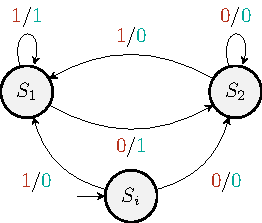
\includegraphics{./imagenes/machineMealy.pdf}
		\caption{Diagrama de estados para una Máquina de Mealy simple, con una entrada, y una salida}
		\label{fig:machineMealy}
	\end{figure}
	
	\begin{table}[h]
		\centering
		\bgroup
		\def\arraystretch{1.5}
		\begin{tabular}{|c|c|c|c|}
			\hline
			Estado actual & entrada & Siguiente estado & Salida \\
			\hline
			\multirow{2}{*}{$S_{i}$} & 0 & $S_{0}$ & \multirow{2}{*}{0} \\
			\cline{2-3}
			& 1 & $S_{1}$ &  \\
			\hline
			\multirow{2}{*}{$S_{0}$} & 0 & $S_{0}$ & 0 \\
			\cline{2-4}
			& 1 & $S_{1}$ & 1 \\
			\hline
			\multirow{2}{*}{$S_{1}$} & 0 & $S_{0}$ & 1 \\
			\cline{2-4}
			& 1 & $S_{0}$ & 0 \\
			\hline
		\end{tabular}
		\egroup
		\caption{Tabla de transición de un \textit{XOR} de las últimas 2 entradas}
		\label{tab:tableMealy}
	\end{table}
	
	Los verificadores de tiempo se utilizan para verificar que en cierto intervalo de tiempo, la señal se debe mantener estable, antes y después de que la entrada del clock cambie.
	
	\vspace{10mm}
	
	\begin{itemize}
		\item Setup time: Es la cantidad de tiempo en el que la señal sincronizada debe estar estable antes que el clock tenga un cambio, para garantizar que los datos se guarden/transmitan exitosamente, este valor puede ser modificado, variando el periodo en el clock.
		\item Hold time: Es la cantidad de tiempo en que la señal se mantiene estable después de haber tenido el cambio y haber pasado el borde del clock. Este también garantiza que los datos se guarden/transmitan exitosamente. 
	\end{itemize}
	
	\begin{figure}[h]
		\centering
		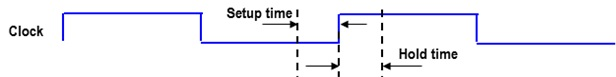
\includegraphics[width=\linewidth]{./imagenes/setup_hold.jpg}
		\caption{Setup Time \& Hold Time \cite{rebote}}
		\label{fig:setup-time}
	\end{figure}
	
	
	Los elementos mecánicos como botones, teclas o interruptores, son dispositivos que cierran o abren un circuito mediante el contacto entre dos superficies metálicas, tal y como se muestra en la siguiente figura.
	
	\begin{figure}[hbtp]
		\centering
		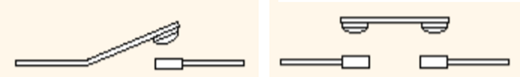
\includegraphics[scale = 0.4]{imagenes/rebote.png}
		\caption[Figura1]{Dispositivos mecánicos \cite{rebote}}
		\label{fig:DispMeca}
	\end{figure}
	
	Dichas superficies metálicas, poseen elasticidad, de manera que al ponerlas en contacto se genera un choque que produce un movimiento en sentido contrario que las aleja, lo cual, sucede repetidamente hasta que se disipa la energía cinética adquirida por la lámina en movimiento, a este fenómeno se le conoce como efecto rebote.
	El efecto rebote se presenta por el hecho de que la apertura o el cierre del circuito no es instantáneo, por lo que durante un intervalo de tiempo oscila entre cerrado y abierto.
	
	\begin{figure}[hbtp]
		\centering
		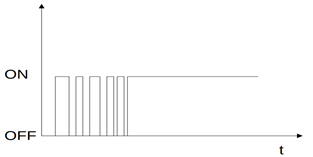
\includegraphics[scale = 0.5]{imagenes/efectoRebote.png}
		\caption[Figura1]{Dispositivos mecánicos \cite{rebote}}
		\label{fig:EfectoRebo}
	\end{figure}
	
	
	En el caso de los circuitos digitales, también existen soluciones para este problema, por ejemplo, se puede hacer un circuito anti-rebote, de manera que se utilizan componentes como un Flip-Flop tipo  R-S, de manera que, si se tienen ambas entradas conectadas a la tierra, con resistencias, se puede cambiar su salida como respuesta a un cambio en una de sus entradas, pero como los flips-flops tienen el efecto de memoria, no importa, porque su estado se mantiene igual a que si solo hubiera entrada un pulso de 1 a 0, hasta que se haga m\'as estable, también se usan compuertas l\'ogicas , especialmente las de "smith-trigger", ya que son mucho mas estables.
	
	\begin{figure}[h]
		\centering
		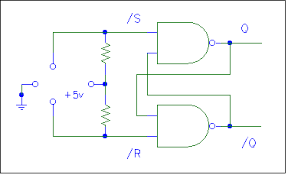
\includegraphics[scale=0.6]{imagenes/flipflopsrebote.png}
		\caption{Ejemplo Solución Flip-Flop \cite{rebote}}
		\label{fig:tikz-flipflop}
	\end{figure}
	
	\begin{figure}[h]
		\centering
		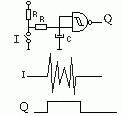
\includegraphics[scale=0.7]{imagenes/smith.png}
		\caption{Ejemplo solución con smith-trigger \cite{rebote}}
		\label{fig:tikz-smith}
	\end{figure}
	
	\begin{figure}[h]
		\centering
		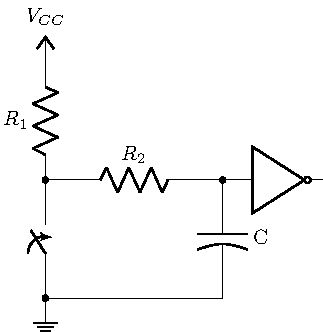
\includegraphics[scale=0.8]{imagenes/rc_debouncer.pdf}
		\caption{Circuito RC para remover oscilación de señal}
		\label{fig:tikz-debouncer}
	\end{figure}
	
	Las señales de sincronización de una interfaz VGA son las que se detallan en la tabla 1. R, G y B son tres señales analógicas que que determinan el color de un punto en la pantalla. Por otra parte, $h_sync$ y $v_sync$ son las señales que determinan la posición de referencia de la pantalla donde debe ser mostrado el punto.
	
	\begin{table}[h]
		\centering
		\begin{tabular}{||c|c|c||}
			\hline
			\hline
			Pin & Señal       & Descripción \\
			\hline
			1   & R           & análogo rojo, 0-0.7 V\\
			2   & G           & análogo verde, 0-0.7 V o 0-3.1 V si sync-on-green \\
			3   & B           & análogo azul, 0-0.7 V\\
			13  & $h_{sync}$  & horizontal sync, 0V/5V waveform\\
			14  & $v_{sync}$  & vertical sync, 0V/5V waveform\\
			\hline
			\hline
		\end{tabular}
		\caption{Tabla de transiciones}
		\label{tab:VGA}
	\end{table}
	
	Mediante un manejo correcto de estas señales según las especificaciones de sincronización de la VGA, es posible mostrar lo que se desee en la pantalla. 
	
	Un diagrama de tiempos de las señales de sincronización de VGA para una resolución de 640x480 píxeles esta dado de la forma:
	
	\begin{figure}[hbtp]
		\centering
		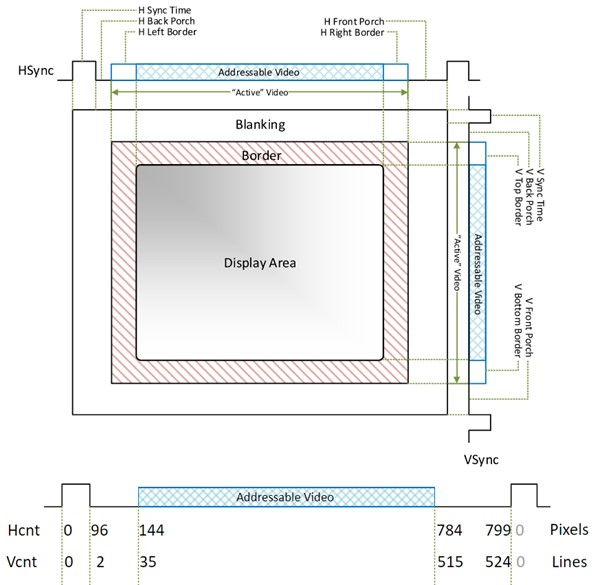
\includegraphics[width = \columnwidth]{imagenes/vgapic.jpg}
		\caption[Figura1]{VGA \cite{vga}}
		\label{fig:VGA}
	\end{figure}
	
	De esta manera para la sincronización horizontal se tiene: 
	\begin{itemize}
		\item $H Sync Time = 3.813 \mu s$
		\item $H Back Porch = 1.907 \mu s$
		\item $H Front Porch = 0.636 \mu s$
		\item $H Addr Video Time = 25.422 \mu s$
		\item $H L/R Border = 0 \mu s$
		\item $Total = 31.778 \mu s$
	\end{itemize}
	
	Realizando el calculo de la frecuencia tenemos:
	
	\begin{equation}
		f_{H} = \frac{1}{31.778 \mu s} = 31.468 kHz
	\end{equation}
	
	Y para la sincronización vertical se tiene: 
	\begin{itemize}
		\item $V Sync Time = 0.064 ms$
		\item $V Back Porch = 1.048 ms$
		\item $V Front Porch = 0.318 ms$
		\item $V Addr Video Time = 15.253 ms$
		\item $V T/B Border = 0 ms$
		\item $Total = 16.683 ms$
	\end{itemize}
	
	Realizando el calculo de la frecuencia tenemos:
	
	\begin{equation}
		f_{H} = \frac{1}{16.683 ms} = 59.94 Hz
	\end{equation}
	
	\begin{itemize}
		\item Front Porch: Es una región en blanco de la señales de sincronización horizontal y vertical, que se presenta antes de la región activa de vídeo.
		\item Back Porch: Es una región en blanco de la señales de sincronización horizontal y vertical, que se presenta después de la región activa de vídeo.
	\end{itemize}
	
	\section{Sistema Desarrollado}
	
	\subsection{Experimento 1}
	En este experimento, se requiere realizar ...
	
	\begin{figure}[hbtp]
		\centering
		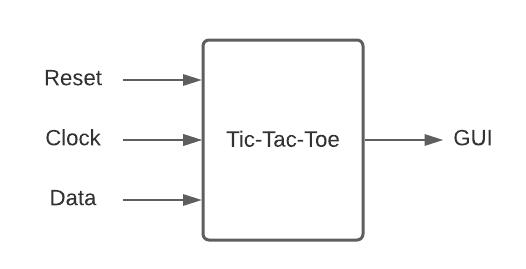
\includegraphics[width = \columnwidth]{imagenes/PrimerN.png}
		\caption[Figura1]{Diagrama de primer nivel de Tic-Tac-Toe.}
		\label{fig:PrimerN}
	\end{figure}
	
	
	\begin{figure}[hbtp]
		\centering
		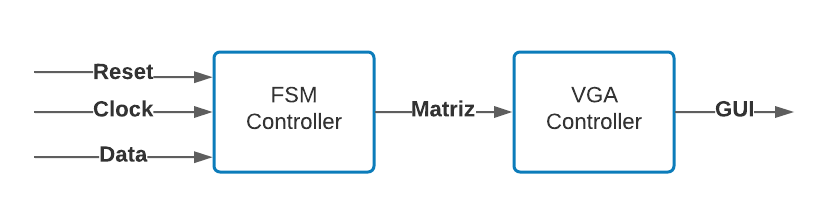
\includegraphics[width = \columnwidth]{imagenes/SegundoN.png}
		\caption[Figura1]{Diagrama de segundo nivel de Tic-Tac-Toe.}
		\label{fig:SegundoN}
	\end{figure}
	
	
	\begin{figure}[hbtp]
		\centering
		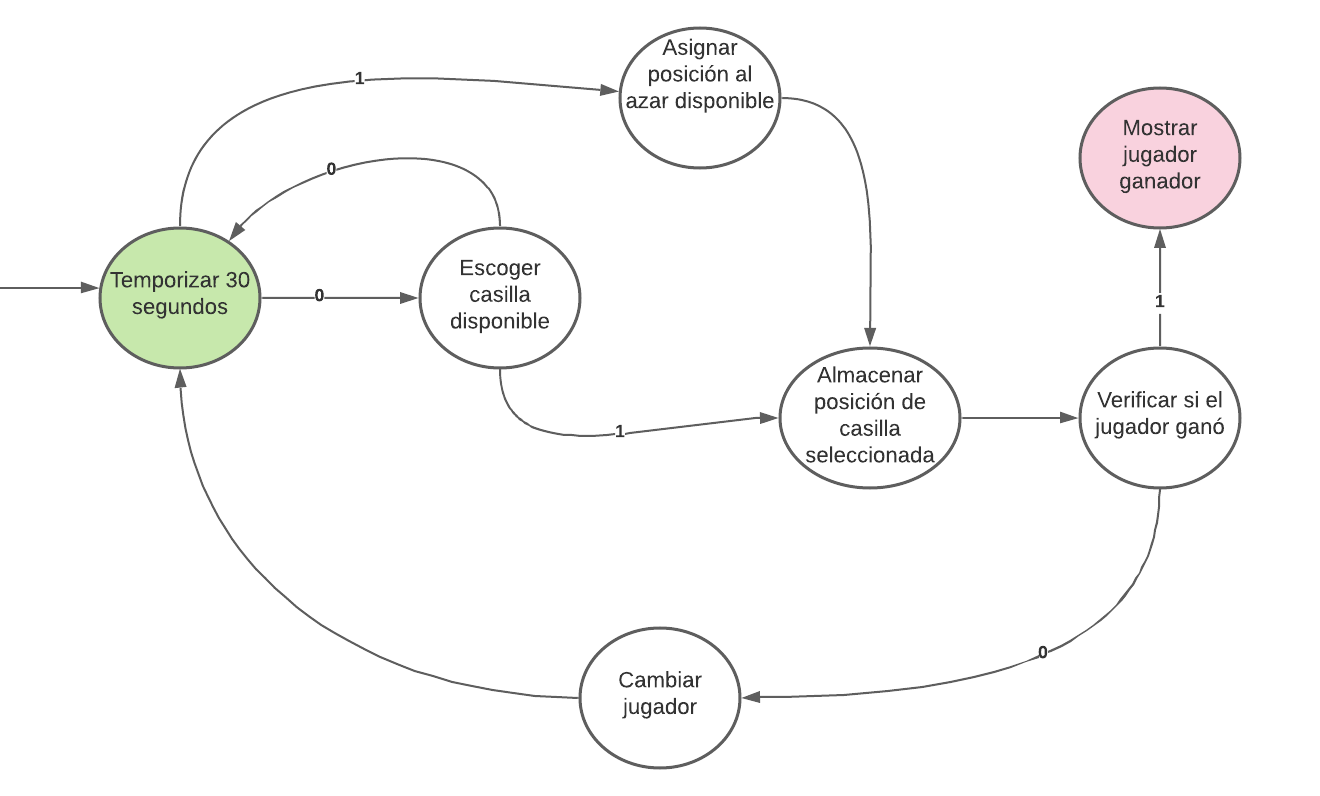
\includegraphics[width = \columnwidth]{imagenes/MaqEst.png}
		\caption[Figura1]{Maquina de estados del programa.}
		\label{fig:MaqEst}
	\end{figure}
	
	En la figura  \ref{fig:MaqEst}, se puede observar la máquina de estados del sistema, se requieren 3 flip flops a lo interno para poder implementar una máquina como estas ya que al componerse de 7 estados, con 3 flip flops alcanza para poder trabajar con ella. El estado $000$ es el Temporizador de 30 segundos, este es el estado inicial, ya que en cada una una vez que empieza la jugada, se deben empezar a contabilizar estos 30 segundos. El estado $001$ es Escoger casilla disponible, la función de este estado es permitirle al jugador escoger una casilla disponible en la cuadrícula, si aún no pasan los 30 segundos. El estado $010$ es Asignar posición al azar disponible, la función de este estado es la de asignar a un jugador una posición en la cuadrícula del juego disponible, si este no seleccionó ninguna, pasados los 30 segundos. El estado $011$ es Almacenar posición de casilla seleccionada, su función es actualizar el vector de las posiciones de las casillas, con la que fue seleccionada, ya sea por el jugador o de manera aleatoria por el sistema. El estado $100$ es Verificar si el jugador ganó, su función es verificar entre las jugadas permitidas ganadoras, y ver si el jugador con la selección de casilla anterior, generó alguna jugada ganadora. El estado $101$ es Cambiar jugador, su función es asignarle el turno al siguiente jugador, en caso de que el que estaba jugando la partida, no haya generado una partida ganadora. Y finalmente, el estado $110$  es Mostrar jugador ganador, este estado es el encargado de enviarle una señal al controlador de VGA, para indicarle que el jugador que está realizando dicha jugada, fue el ganador, ya que cumplió con alguna de las formas para poder ganar el juego (línea horizontal, línea vertical o diagonal).
	
	\section{Resultados}
	
	Al realizar este laboratorio, se obtuvo la máquina de estados que se observa en la Figura \ref{fig:MaqR1}, generada al visualizar el diagrama de bloques de todo el sistema en RTL Simulation.
	
	\begin{figure}[hbtp]
		\centering
		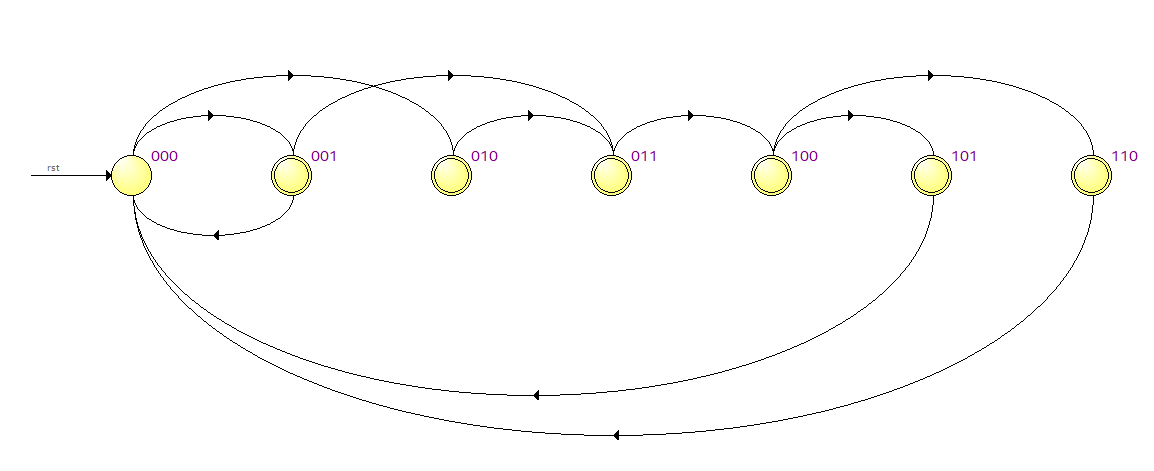
\includegraphics[width = \columnwidth]{imagenes/MaqR1.png}
		\caption[Figura1]{Máquina de estados del programa generada por RTL Simulation.}
		\label{fig:MaqR1}
	\end{figure}
	
	En esta máquina se puede observar como se cumple la lógica del juego descrita en la Figura \ref{fig:MaqEst}.
	
	Posteriormente, en la Figura \ref{fig:MaqE1}, se puede observar la máquina de estados encargada de cambiar de jugador, esta se debió implementar para tener una lógica secuencial en el proceso de asignar el turno a cada jugador, e intercalarlos.
	
	\begin{figure}[hbtp]
		\centering
		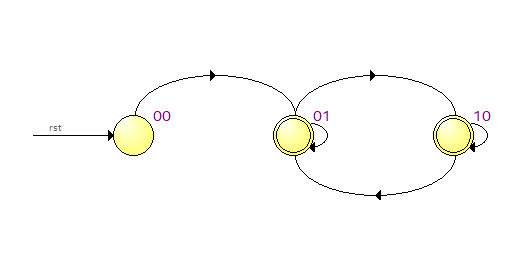
\includegraphics[width = \columnwidth]{imagenes/MaqE1.png}
		\caption[Figura1]{Máquina de estados para cambiar de jugador, generada por RTL Simulation.}
		\label{fig:MaqE1}
	\end{figure}
	
	En la Figura \ref{fig:timer}, se puede observar el testbench generado al comprobar el funcionamiento del temporizador, este módulo es el encargado de contar los 30 segundos, sincronizado a la señal de reloj de todo el sistema.
	
	\begin{figure}[hbtp]
		\centering
		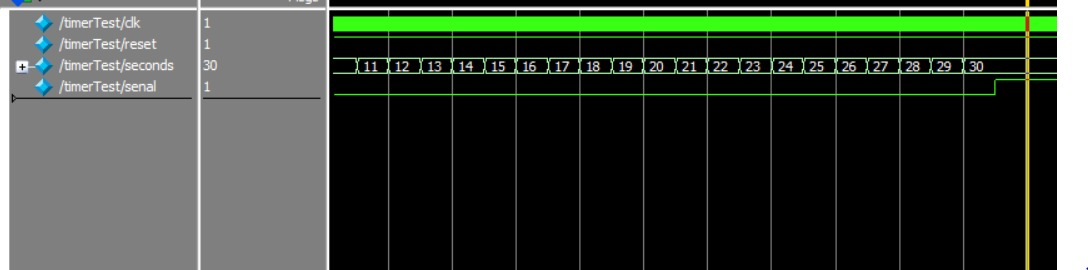
\includegraphics[width = \columnwidth]{imagenes/timer.jpeg}
		\caption[Figura1]{Testbench del temporizador.}
		\label{fig:timer}
	\end{figure}
	
	
	En la Figura \ref{fig:cou}, se puede observar el testbench generado para comprobar el adecuado funcionamiento del contador de 1 a 9. Este módulo es el que es utilizado para asignar a la casilla correspondiente, su respectivo valor.
	
	\begin{figure}[hbtp]
		\centering
		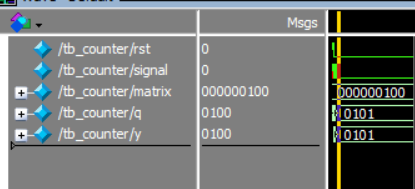
\includegraphics[width = \columnwidth]{imagenes/cou.png}
		\caption[Figura1]{Testbench del contador.}
		\label{fig:cou}
	\end{figure}
	
	En la Figura \ref{fig:ran}, se puede observar el testbench del módulo Random, el cual se encarga de asignar una posición de casilla random disponible, en caso de que pasen los 30 segundos y el jugador no haya seleccionado una casilla disponible.
	
	
	\begin{figure}[hbtp]
		\centering
		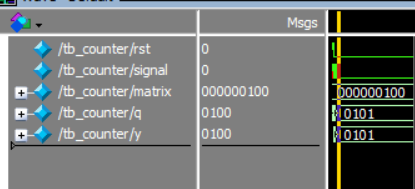
\includegraphics[width = \columnwidth]{imagenes/cou.png}
		\caption[Figura1]{Testbench del Random.}
		\label{fig:ran}
	\end{figure}
	
	En la Figura \ref{fig:play}, se puede observar el testbench de la máquina de estados de los jugadores, en donde el estado $01$ es para el jugador 1 y el estado $10$, para el jugador 2; dicha máquina va a estar operando entre ambos estados, y cuando un jugador selecciona una casilla disponible, le da el turno al siguiente jugador para que escoja su respectiva casilla.
	
	\begin{figure}[hbtp]
		\centering
		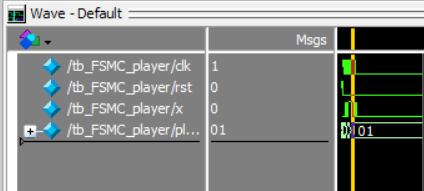
\includegraphics[width = \columnwidth]{imagenes/player.png}
		\caption[Figura1]{Testbench de la máquina de estados para cambiar de jugador.}
		\label{fig:play}
	\end{figure}
	
	\section{Análisis de Resultados}
	
	Al implementar la lógica de la máquina de estados con el controlador VGA, existieron dos módulos los cuales no pudieron ser implementados con toda la lógica del programa: el timer, el cual se observa en la Figura \ref{fig:timer} y el cual funciona adecuadamente por separado y con su respectivo testbench se puede ver su adecuado funcionamiento. Y por consiguiente el random, ya que no existe la señal que se genera por el temporizador al llegar a los 30 segundos para poner en alto su salida y así activar el módulo random, el cual se encarga de asignar una posición aleatoria de 1 a 9, sobre la posición que el sistema le asigna al jugador.
	
	A su vez el módulo principal que contiene la lógica del juego está compuesto por otros módulos como:
	
	\begin{itemize}
		\item Contador: este se encarga de cambiar de posición buscando el jugador en turno la posición deseada para realizar jugada, su funcionamiento es correcto ya que como se comprobó en las pruebas realizadas realiza su función.
		\item Maquina estados cambiar jugador: en esta se diseño la lógica para realizar los cambios de turno entre un jugador y otro, su funcionamiento no es del todo correcto ya que en ocasiones al iniciar una partida realiza una doble jugada para el jugador inicial.
		\item Memoria de las casillas: en este modulo se implemento una memoria de registros para cada casilla del tic tac toe, el funcionamiento de este es el deseado ya que conserva la información de las jugadas realizadas previamente y a su vez no permite que se dibuje o se realice otra jugada sobre una casilla previamente utilizada.
		\item Seleccionar posición: la función de este modulo es que cuando el jugador se encuentre en la casilla deseada para realizar la jugada deseada, al seleccionar que se desea realizar en esa casilla funciona de acuerdo a lo planteado ya que con ayuda de otros módulos imprime la imagen deseada según el jugador de turno.
		\item Maquina de estados de la lógica del juego: esta maquina se encarga de realizar la conexión de señales entre los otros módulos que funcionan para la lógica del juego, su funcionamiento no es del todo el deseado ya que en ocasiones no conecta bien con el modulo de cambiar de jugador y le asigna un doble turno al jugador inicial, además no se encuentra conectada con el temporizador que determina la jugada random después el tiempo de espera de 30 segundos.
	\end{itemize}
	
	Por otro lado la implementación del controlador VGA funciona correctamente, ya que la sincronización con los ciclos de reloj y la carga de las imágenes desde un sprite en memoria, estas a su vez se instancia en un módulo dentro del controlador del VGA, finalmente se muestran en pantalla como se desea, sin embargo cabe recalcar que sin motivo conocido el fondo de las cuadrículas del tic tac toe brinca colores diferentes según la pantalla en la que se esté utilizando.
	
	\section{Conclusiones}
	Al final dicho laboratorio, se obtuvieron las siguientes conclusiones:
	
	\begin{itemize}
		\item Las máquinas de estado finito proporcionan una forma sistemática de diseñar circuitos secuenciales dada una función específica. 
		
		\item Los controladores VGA aunque son fáciles de implementar presentan la desventaja de tener bajas resoluciones, además que la señal que emiten es de tipo analógica y al querer emitir señales digitales puede ocasionar problemas.
		
		\item Al momento de implementar soluciones complejas, las cuales se componen de varios componentes más pequeños y sencillos, lo óptimo es modularizar la propuesta, trabajando por medio del modelo estructural.
		
		\item Es necesario que todos los módulos del sistema operen bajo la misma señal de reloj, para este caso a 25MHz.
		
		\item Al crear máquinas de estado combinacionales, se puede comprobar mediante su correspondiente diagrama de estados, el adecuado funcionamiento de la misma y que corresponda al diseño original que fue desarrollado antes de programar la máquina.
		
		
	\end{itemize}
	
	\bibliographystyle{IEEEtran}
	\begin{thebibliography}{1}
		
		
		\bibitem{ddcaarm}
		Harris, S. Harris, D. \emph{Digital Design and Computer Architecture: ARM Edition}. Morgan Kaufmann, 2015.
		
		\bibitem{morse}
		\emph{International Morse code Recommendation ITU-R M.1677-1}. itu.int. International Telecommunication Union. October 2009. Archived from the original on 6 November 2012. Recuperado el 27 de abril del 2021.
		
		\bibitem{wolfram}
		Wolfram, S. \emph{Starting From Randomness}. A New Kind of Science. Wolfram Media, p. 958. 2002. Recuperado el 27 de abril del 2021.
		
		\bibitem{basharin}
		Basharin G. et al. \emph{The Life and Work of A. A. Markov}. Linear Algebra and its Applications 386: 3-26. 2004. Recuperado el 27 de abril del 2021.
		
		\bibitem{rebote}
		Fing.edu.uy. T\'ecnicas de Manejo de E/S. Taller de Firmware. Facultad de Ingenier\'ia.
		\url{https://www.fing.edu.uy/inco/cursos/firmware/teorico/clase05-manejoES.pdf}
		
		\bibitem{vga}
		C. hardware?, J. Beckwith and S. Pefhany, "Can reading VGA signals from my computer harm the hardware?", Electrical Engineering Stack Exchange, 2021. Disponible: https://electronics.stackexchange.com/questions/166757/can-reading-vga-signals-from-my-computer-harm-the-hardware. Recuperado el 27 de abril del 2021..
		
	\end{thebibliography}
\end{document}